% !TEX program = lualatex
\documentclass[border=6pt]{standalone}
% ---------------------------------------------------------------------------
% tikzpreamble.tex -- shared by main.tex and by every standalone in tikz/
% ---------------------------------------------------------------------------
\usepackage{amsmath}
\usepackage{amssymb}
\usepackage{tikz}
\usepackage{circuitikz}
\usetikzlibrary{arrows.meta,calc,positioning,decorations.pathmorphing,decorations.pathreplacing,
                decorations.markings,patterns,angles,quotes,fit,
                shapes.geometric,shapes.misc,backgrounds,intersections}

\ctikzset{bipoles/length=0.85cm}
\ctikzset{resistors/scale=0.85}
\ctikzset{capacitors/scale=0.9}

\tikzset{
  wire/.style      = {line width=0.7pt},
  dashedwire/.style= {line width=0.7pt, densely dashed},
  term/.style      = {circle, draw, line width=0.6pt, fill=white,
                      inner sep=0pt, minimum size=4.5pt},
  node dot/.style  = {circle, fill=black, inner sep=0pt, minimum size=4pt},
  boxlabel/.style  = {font=\sffamily\small},
  annot/.style     = {font=\small, align=left},
  phasor/.style    = {-{Stealth[length=3.2mm,width=2.2mm]}, line width=1.1pt},
  thinphasor/.style= {-{Stealth[length=2.6mm,width=1.8mm]}, line width=0.7pt},
  axis line/.style = {-{Stealth[length=2.6mm,width=1.8mm]}, line width=0.6pt},
  guide/.style     = {densely dashed, line width=0.4pt, gray},
}
\usepackage{siunitx}

\definecolor{metalphase}{RGB}{190,240,247}
\begin{document}
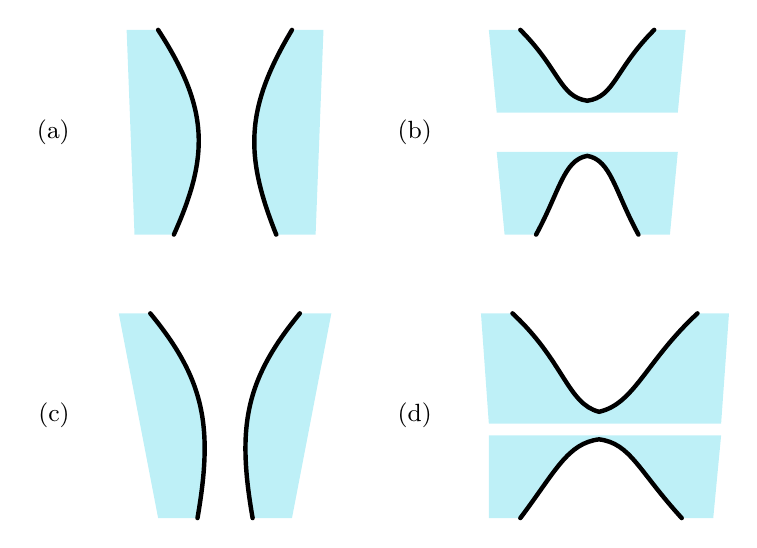
\begin{tikzpicture}[every node/.style={font=\small},
                    boundary/.style={line width=1.6pt,line cap=round}]

  % --- (a) two separated M lakes, temperature T ---------------------------
  \begin{scope}[shift={(0,0)}]
    \fill[metalphase] (-0.15,2.6) .. controls (0.5,1.6) and (0.5,1.0) .. (0.05,0)
        -- (-0.45,0) -- (-0.55,2.6) -- cycle;
    \draw[boundary] (-0.15,2.6) .. controls (0.5,1.6) and (0.5,1.0) .. (0.05,0);
    \fill[metalphase] (1.55,2.6) .. controls (0.95,1.6) and (0.95,1.0) .. (1.35,0)
        -- (1.85,0) -- (1.95,2.6) -- cycle;
    \draw[boundary] (1.55,2.6) .. controls (0.95,1.6) and (0.95,1.0) .. (1.35,0);
    \node[anchor=east] at (-1.15,1.3) {(a)};
  \end{scope}

  % --- (b) linked M phase, temperature T ----------------------------------
  \begin{scope}[shift={(4.6,0)}]
    \fill[metalphase] (-0.55,2.6) -- (-0.15,2.6)
        .. controls (0.35,2.1) and (0.35,1.75) .. (0.7,1.7)
        .. controls (1.05,1.75) and (1.05,2.1) .. (1.55,2.6)
        -- (1.95,2.6) -- (1.85,1.55) -- (-0.45,1.55) -- cycle;
    \draw[boundary] (-0.15,2.6) .. controls (0.35,2.1) and (0.35,1.75) .. (0.7,1.7)
        .. controls (1.05,1.75) and (1.05,2.1) .. (1.55,2.6);
    \fill[metalphase] (-0.45,1.05) -- (1.85,1.05) -- (1.75,0) -- (1.35,0)
        .. controls (1.05,0.55) and (1.0,0.95) .. (0.7,1.0)
        .. controls (0.4,0.95) and (0.35,0.55) .. (0.05,0) -- (-0.35,0) -- cycle;
    \draw[boundary] (0.05,0) .. controls (0.35,0.55) and (0.4,0.95) .. (0.7,1.0)
        .. controls (1.0,0.95) and (1.05,0.55) .. (1.35,0);
    \node[anchor=east] at (-1.15,1.3) {(b)};
  \end{scope}

  % --- (c) lakes just touching, temperature T0 = T + T* -------------------
  \begin{scope}[shift={(0,-3.6)}]
    \fill[metalphase] (-0.25,2.6) .. controls (0.45,1.75) and (0.55,1.15) .. (0.35,0)
        -- (-0.15,0) -- (-0.65,2.6) -- cycle;
    \draw[boundary] (-0.25,2.6) .. controls (0.45,1.75) and (0.55,1.15) .. (0.35,0);
    \fill[metalphase] (1.65,2.6) .. controls (0.95,1.75) and (0.85,1.15) .. (1.05,0)
        -- (1.55,0) -- (2.05,2.6) -- cycle;
    \draw[boundary] (1.65,2.6) .. controls (0.95,1.75) and (0.85,1.15) .. (1.05,0);
    \node[anchor=east] at (-1.15,1.3) {(c)};
  \end{scope}

  % --- (d) merged, temperature T0 -----------------------------------------
  \begin{scope}[shift={(4.6,-3.6)}]
    \fill[metalphase] (-0.65,2.6) -- (-0.25,2.6)
        .. controls (0.4,2.0) and (0.45,1.45) .. (0.85,1.35)
        .. controls (1.3,1.45) and (1.45,2.0) .. (2.1,2.6)
        -- (2.5,2.6) -- (2.4,1.2) -- (-0.55,1.2) -- cycle;
    \draw[boundary] (-0.25,2.6) .. controls (0.4,2.0) and (0.45,1.45) .. (0.85,1.35)
        .. controls (1.3,1.45) and (1.45,2.0) .. (2.1,2.6);
    \fill[metalphase] (-0.55,1.05) -- (2.4,1.05) -- (2.3,0) -- (1.9,0)
        .. controls (1.35,0.6) and (1.25,0.95) .. (0.85,1.0)
        .. controls (0.45,0.95) and (0.3,0.6) .. (-0.15,0) -- (-0.55,0) -- cycle;
    \draw[boundary] (-0.15,0) .. controls (0.3,0.6) and (0.45,0.95) .. (0.85,1.0)
        .. controls (1.25,0.95) and (1.35,0.6) .. (1.9,0);
    \node[anchor=east] at (-1.15,1.3) {(d)};
  \end{scope}
\end{tikzpicture}
\end{document}
